%% 
%%	This is file 'beamer_sample.tex'
%%	according to an MPIDR's PowerPoint template (?)
%%	
%%	by Eric Naujoks
%%
%%	Problems, bugs and comments to 
%%	naujoks@demogr.mpg.de
%%

%%%%%%%%%%%%%%%%%%%%%%%%%%%%%%%%%%
%%	Praelegomena								%%
%%%%%%%%%%%%%%%%%%%%%%%%%%%%%%%%%%
%%	- Make sure that you use utf8-encoding for all your .tex-files!!! (TeXnicCenter since version 2.0)
%%	- TeXnicCenter update: MPIDR intranet > Hard- & Sortfware > Software > Script and text editors > TeXnicCenter

\documentclass[20pt]{beamer}

\usepackage[ngerman,english]{babel}
\usepackage{tikz}
\usepackage[normalem]{ulem}
\geometry{paperwidth=10in, paperheight=7.5in}
\usepackage{animate}

\usepackage[utf8]{inputenc}

\usepackage[mpidr]{./mpidr/beamerthemeMPIDR}

%% Declaring title and author
\title{Extensions and applications of \\ the Lexis diagram}
\subtitle{Tim Riffe}		%%

%%	the institute's logo
\renewcommand{\mylogo}{\includegraphics[width=4.7in]{mpidr_logo_colour_en}}
\usepackage{color}
\definecolor{mygray}{rgb}{0.8,0.8,0.8}

\defbeamertemplate{description item}{align left}{\insertdescriptionitem\hfill}
%%	should be the very last package to be loaded
\usepackage{hyperref}

%%%%%%%%%%%%%%%%%%%%%%%%%%%%%%%%%%
%%	Beginning of the document		%%
%%%%%%%%%%%%%%%%%%%%%%%%%%%%%%%%%%
\begin{document}

%%	titlepage - fixed frame:
%%	========================

\begin{frame}
	\titlepage
\end{frame}
%-------------------

% TOC
%\begin{frame}{Plan}
%\tableofcontents
%\end{frame}


%\begin{frame}
%\vspace{-15em}
%\begin{center}
%\hspace*{-6cm}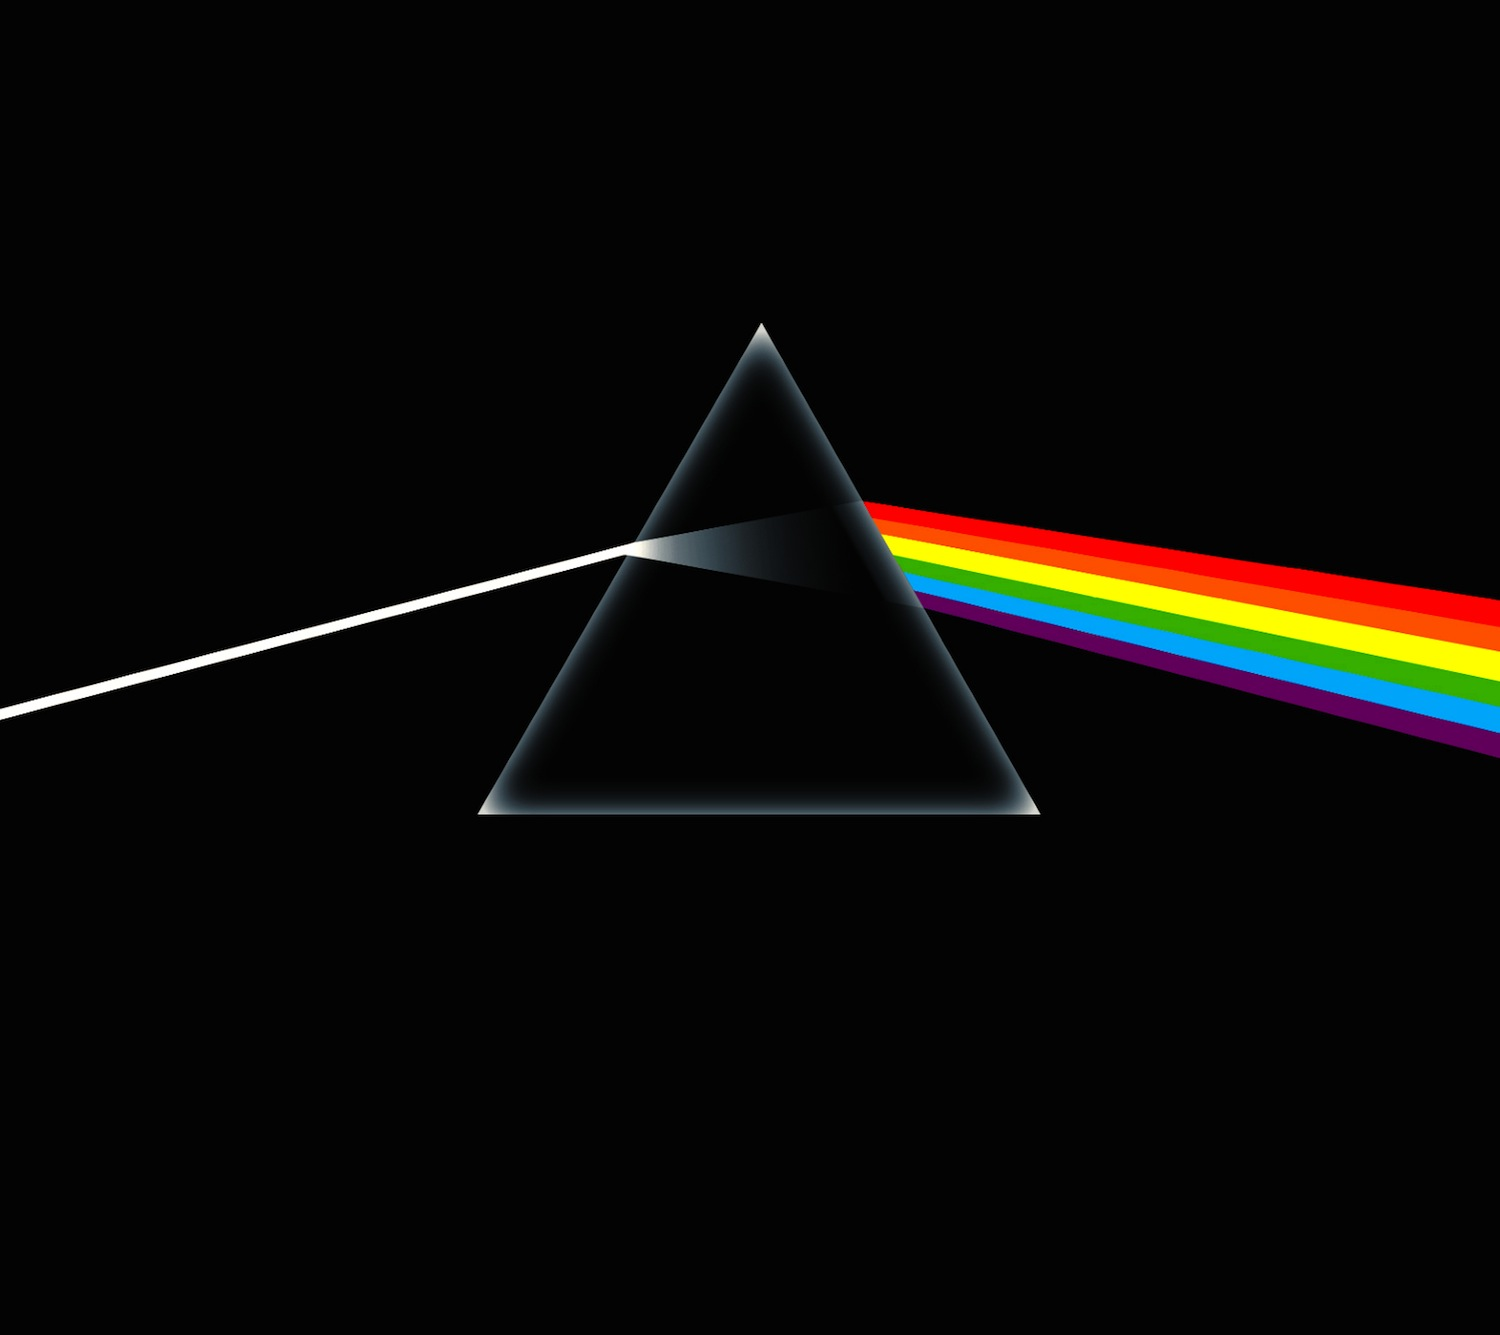
\includegraphics[scale=.7]{Figures/prism.jpg}
%\end{center}
%\end{frame}
%
\section{Standard applications}
%-----------------------------------------


\begin{frame}
\frametitle{Method design I}
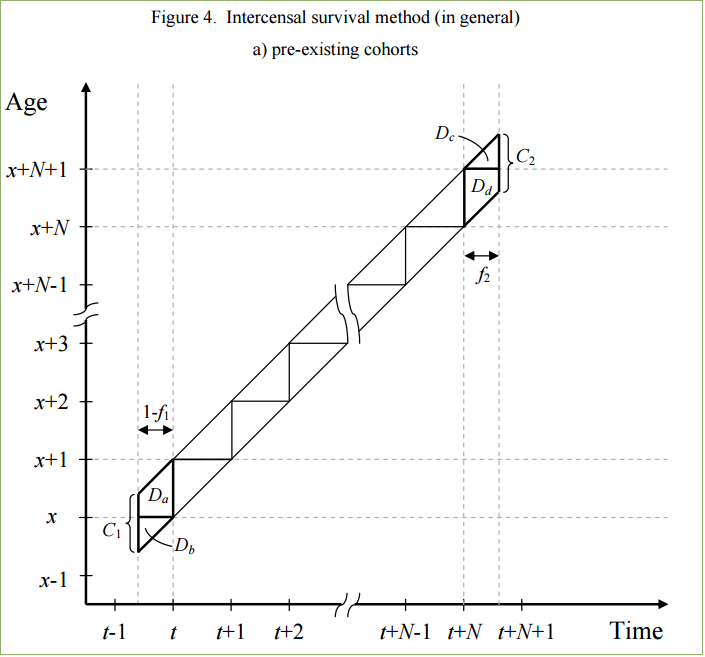
\includegraphics[scale=.65]{Figures/HMD_MPv5Fig4.png}\\
HMD Methods protocol (2007)
\end{frame}

\begin{frame}
\frametitle{Method design II}
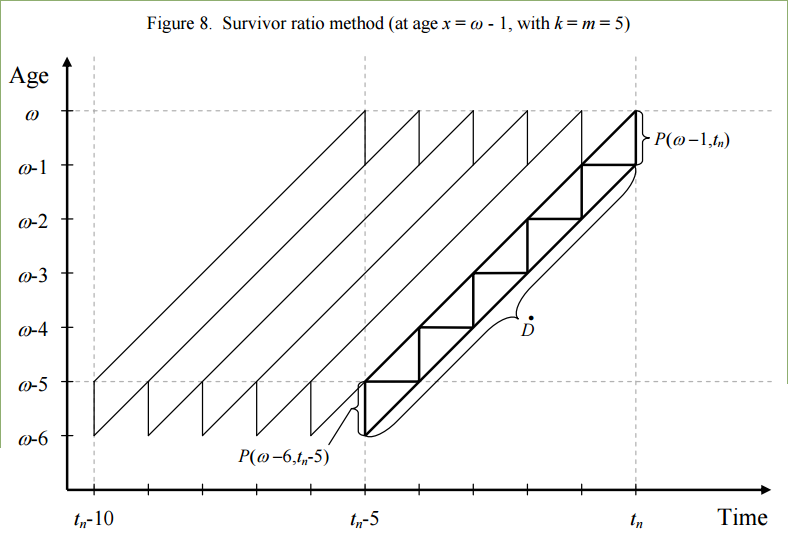
\includegraphics[scale=.7]{Figures/HMD_MPv5Fig8.png}\\
HMD Methods protocol (2007)
\end{frame}

\begin{frame}
\frametitle{Quality and consistency diagnostics I}
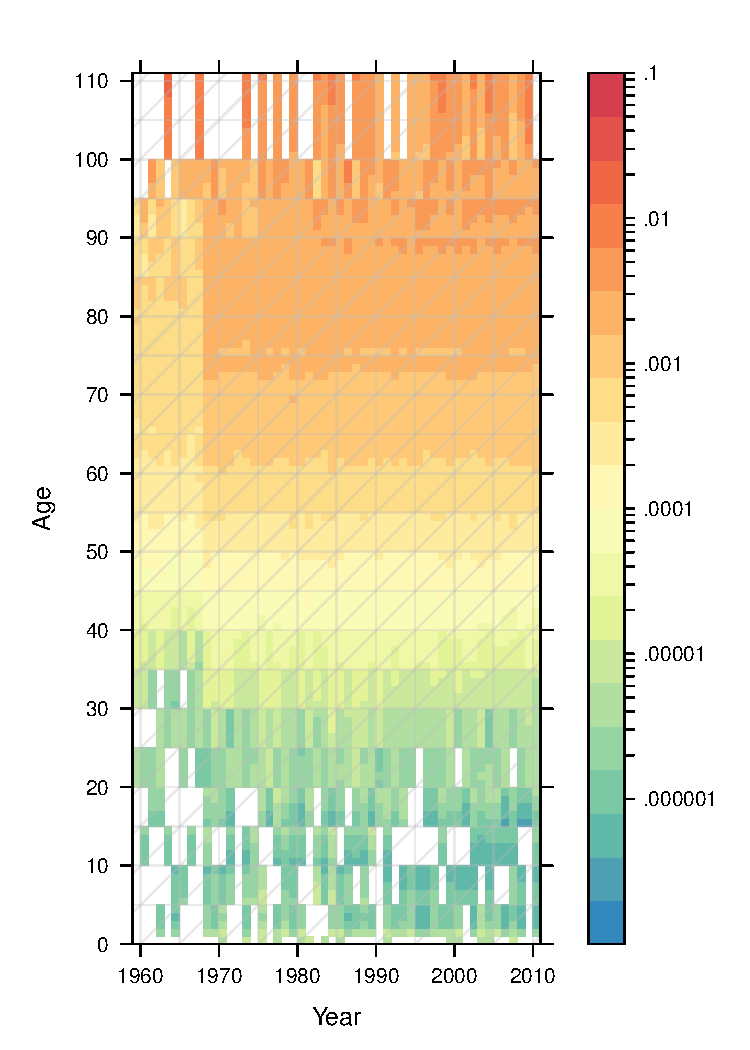
\includegraphics[scale=.8]{Figures/APC_males_CA_cancer.pdf}\\
Data courtesy of HMD: cancer, males, California.
\end{frame}

\begin{frame}
\frametitle{Quality and consistency diagnostics II}
\begin{center}
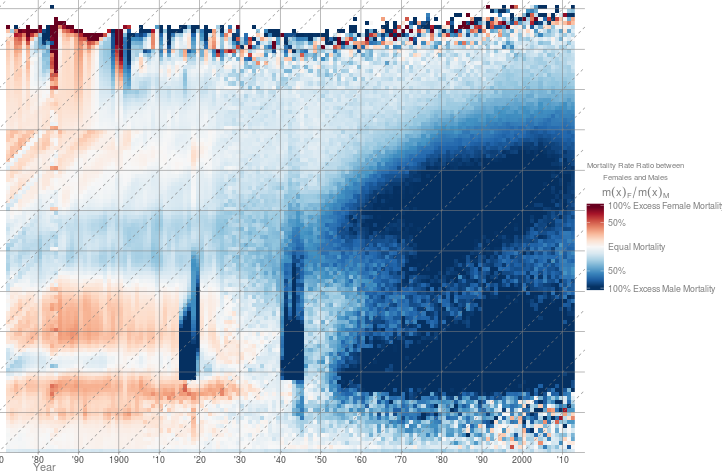
\includegraphics[scale=.8]{Figures/Schoeley2.png}
\end{center}
Sex differences in mortality\\The Human Mortality Explorer, Jonas Schoeley
(2015)
\end{frame}

\begin{frame}
\frametitle{Pattern detection \& storeytelling I}
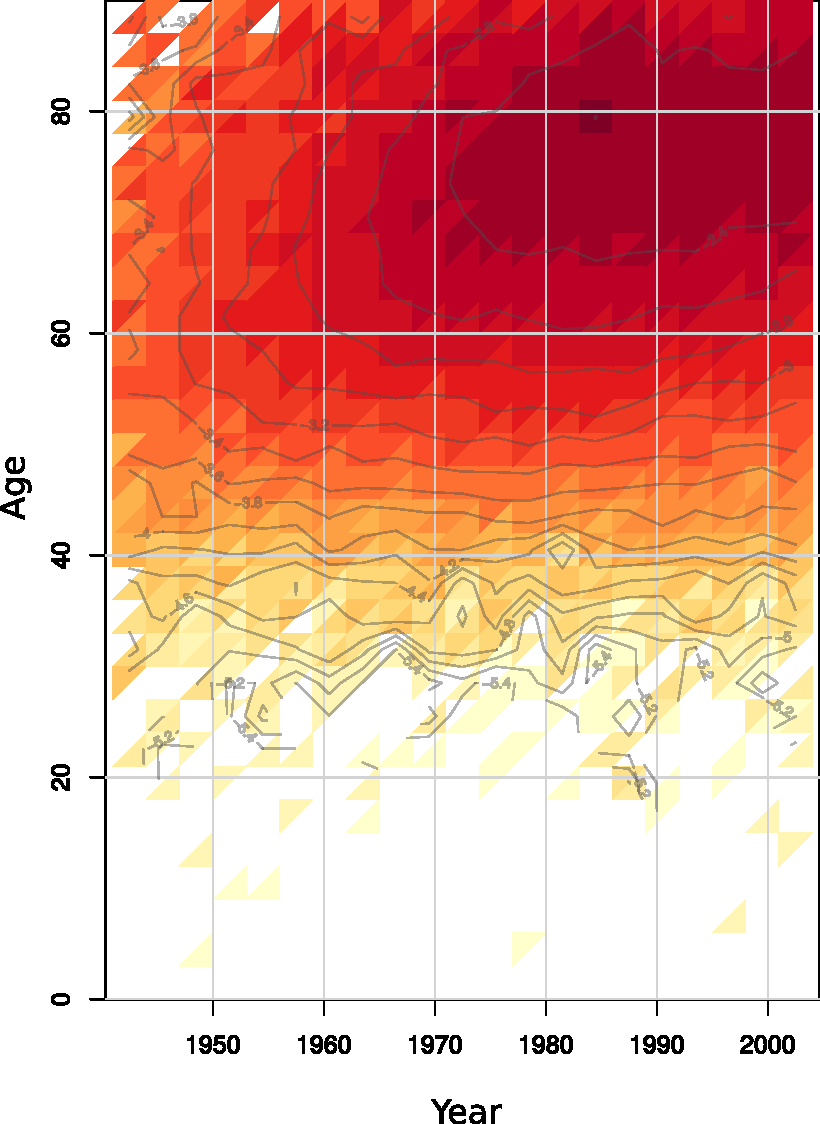
\includegraphics[scale=.7]{Figures/LungCancerDenmark.pdf}\\
Lung cancer mortality, males, Denmark\\
Data courtesy of Bendix Carstensen (2016)
\end{frame}

\begin{frame}
\frametitle{Pattern detection \& storeytelling II}
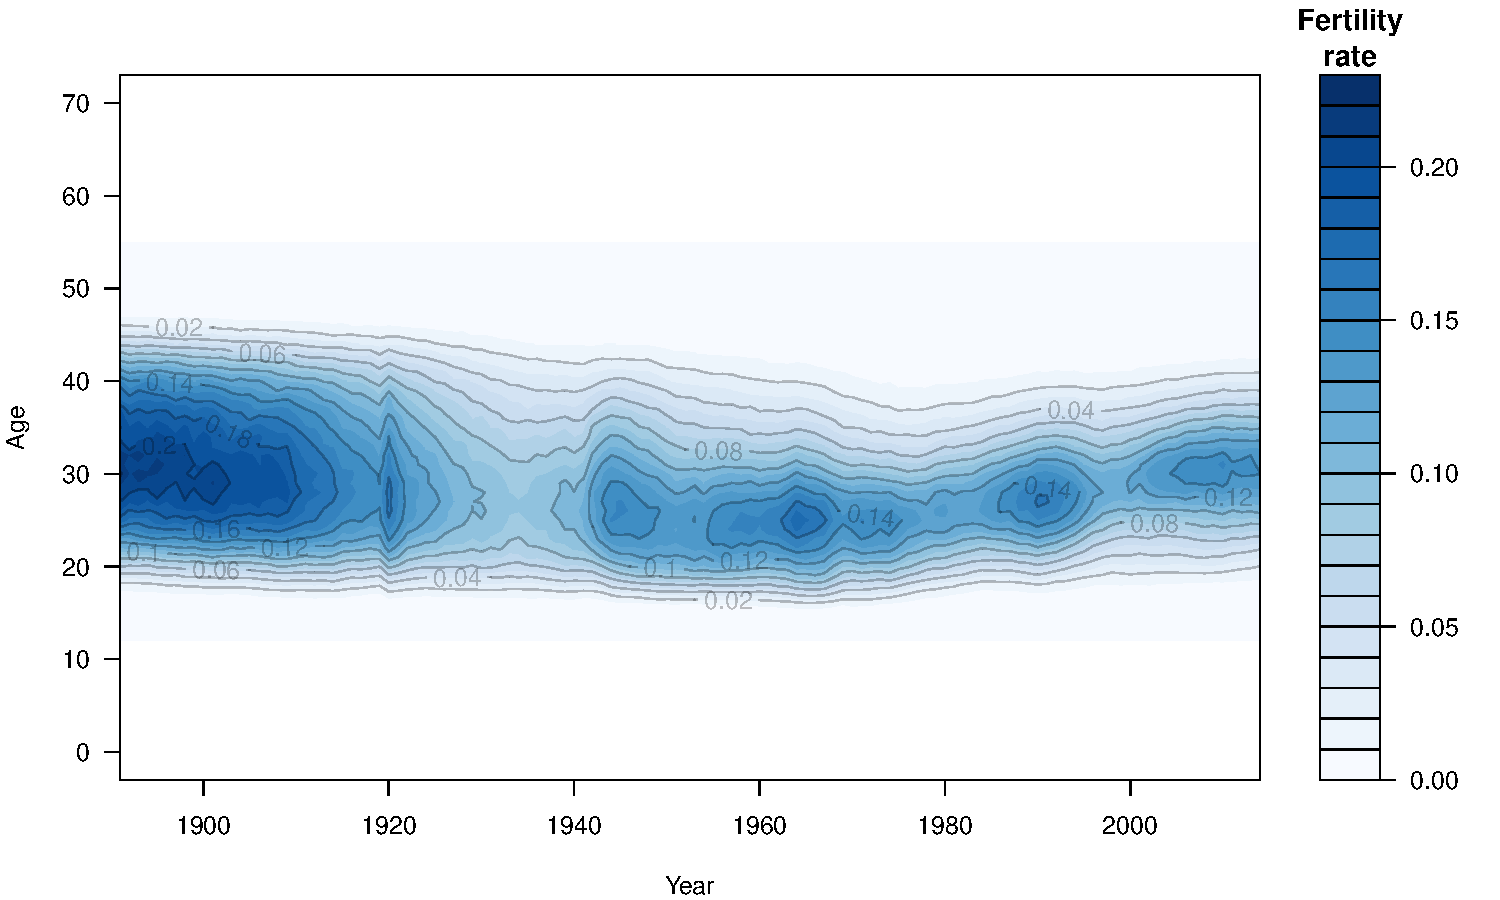
\includegraphics[scale=.85]{Figures/FertAPC.pdf}\\
Sweden fertility, 1891-2014 (HFD)
\end{frame}

%-----------------------------------------
\section{Non-standard applications}
\begin{frame}
\frametitle{Cohort structure and composition}
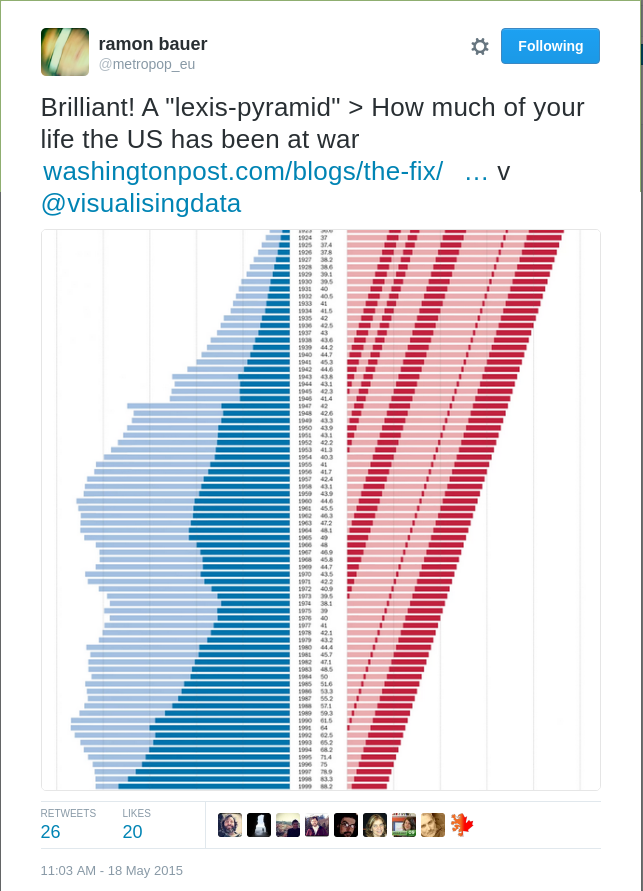
\includegraphics[scale=.55]{Figures/WPLexisPyramid.png}
\end{frame}


\begin{frame}
\frametitle{Subpopulation composition and renewal}
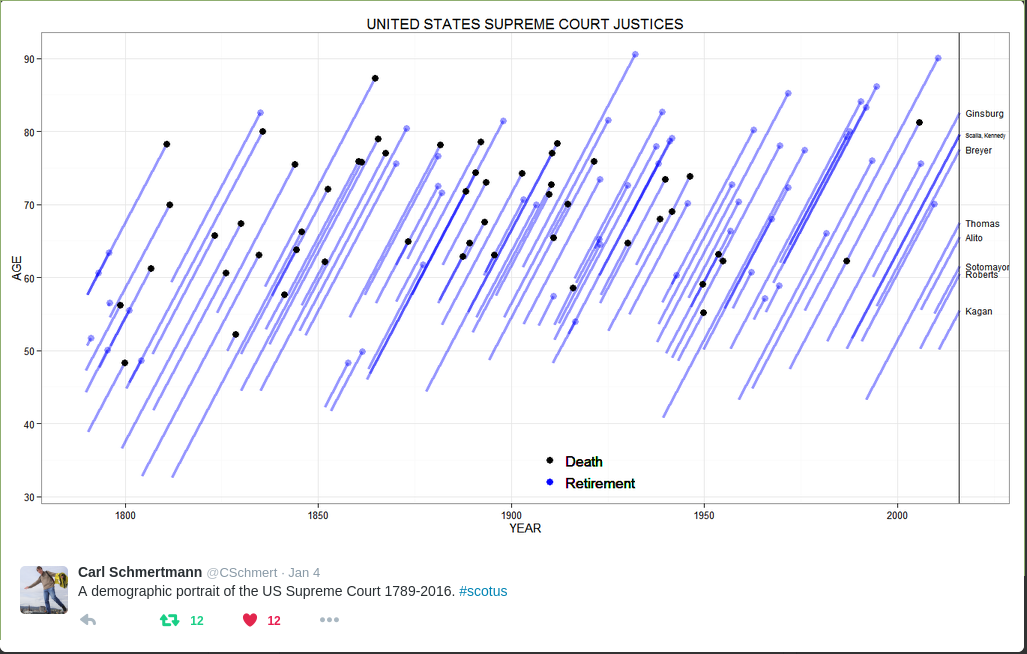
\includegraphics[scale=.65]{Figures/SchmertmannJustices.png}
\end{frame}

\begin{frame}
\frametitle{Defense $=$ birth}
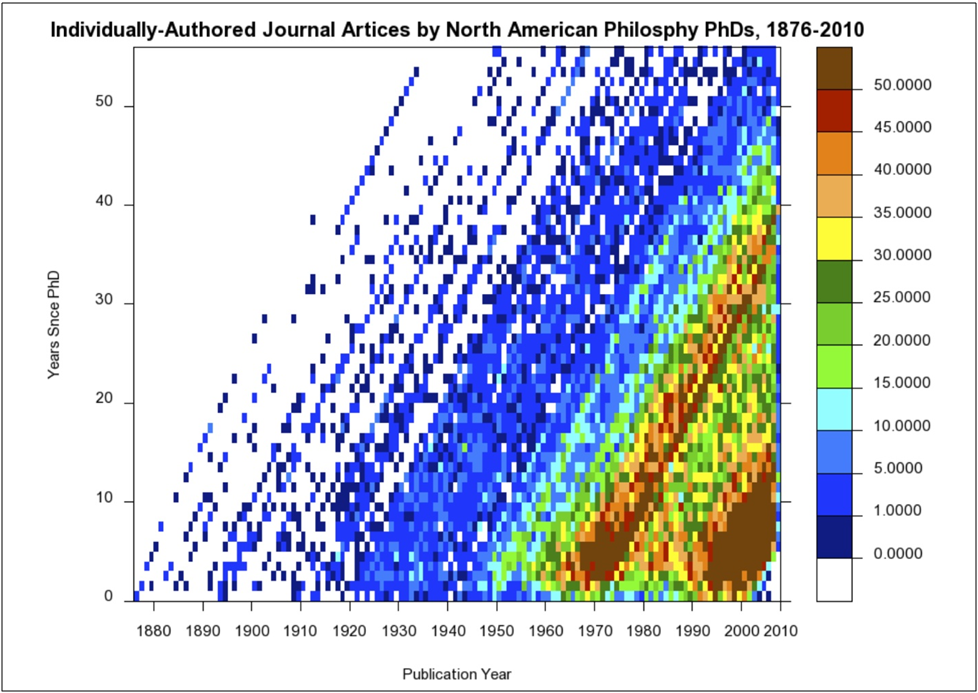
\includegraphics[scale=1.3]{Figures/LexisArticles.png}\\
Sula (2012)
\end{frame}

%%-----------------------------------
%\subsection{aplicaciones no serias}
%\begin{frame}
%\frametitle{adivina que es esto I}
%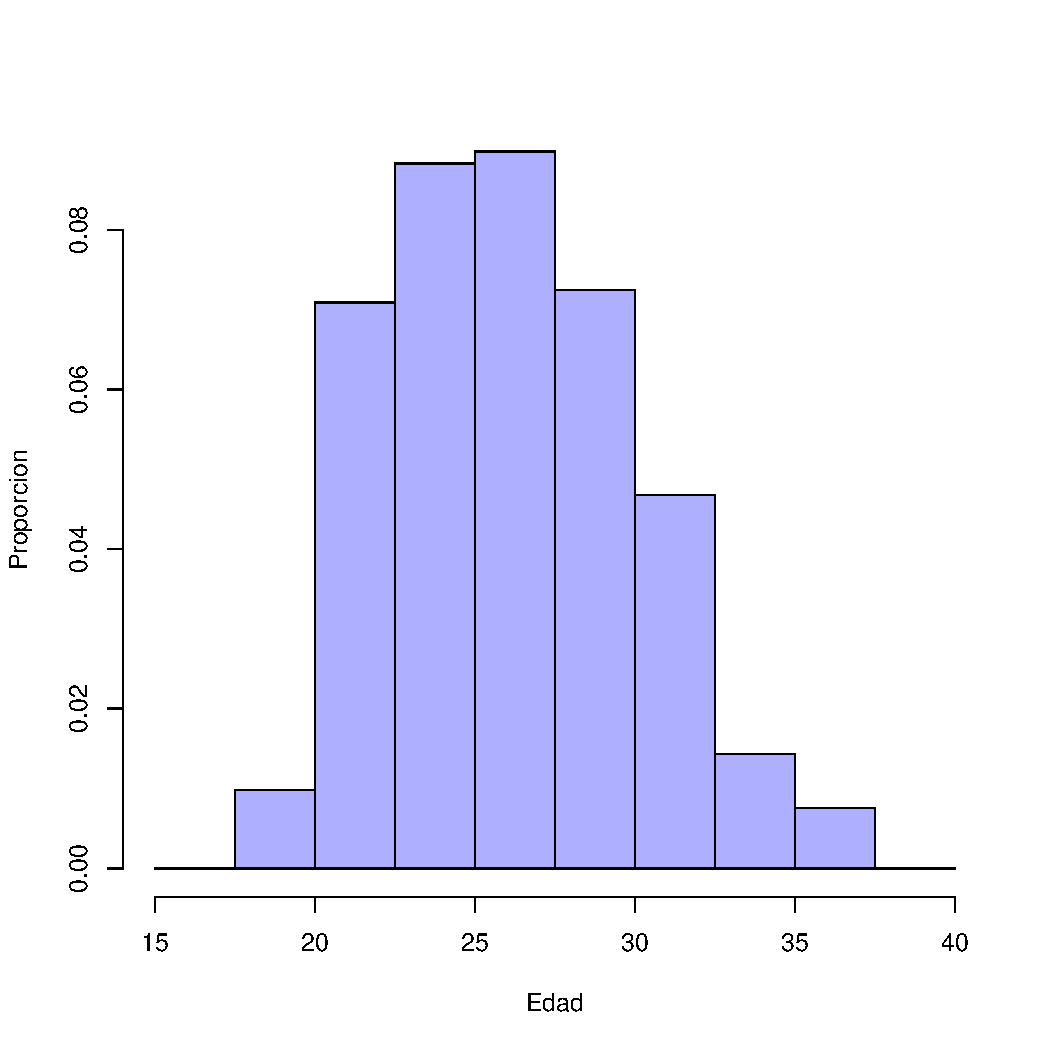
\includegraphics[scale=.8]{Figures/PlayersAges.pdf}
%\end{frame}
%
%\begin{frame}
%\frametitle{adivina que es esto II}
%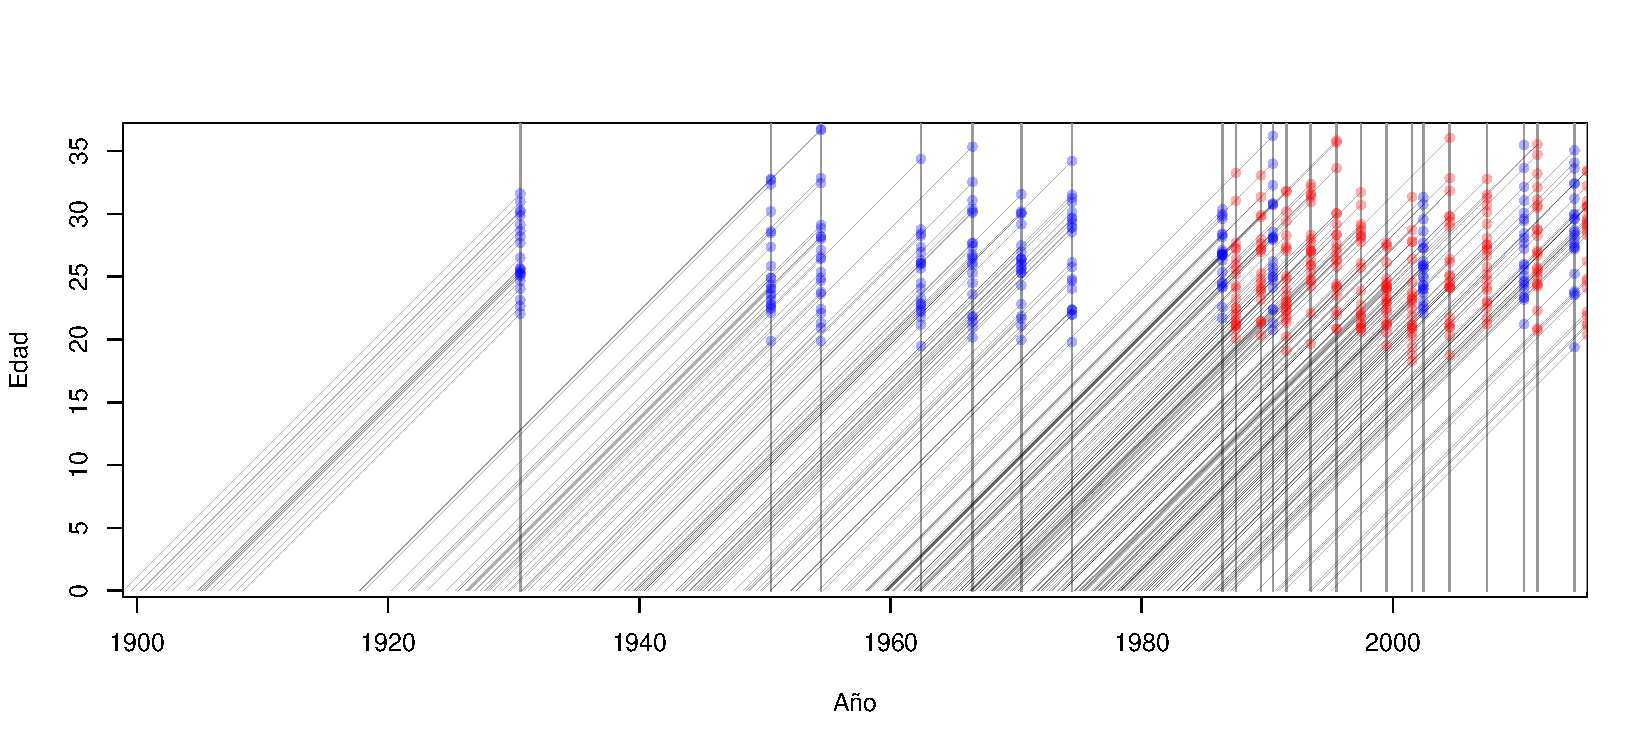
\includegraphics[scale=.88]{Figures/LexisPlayers1.pdf}\\
%datos scraped de Wikipedia
%\end{frame}
%
%\begin{frame}
%\frametitle{o primera entrada como el nacimiento}
%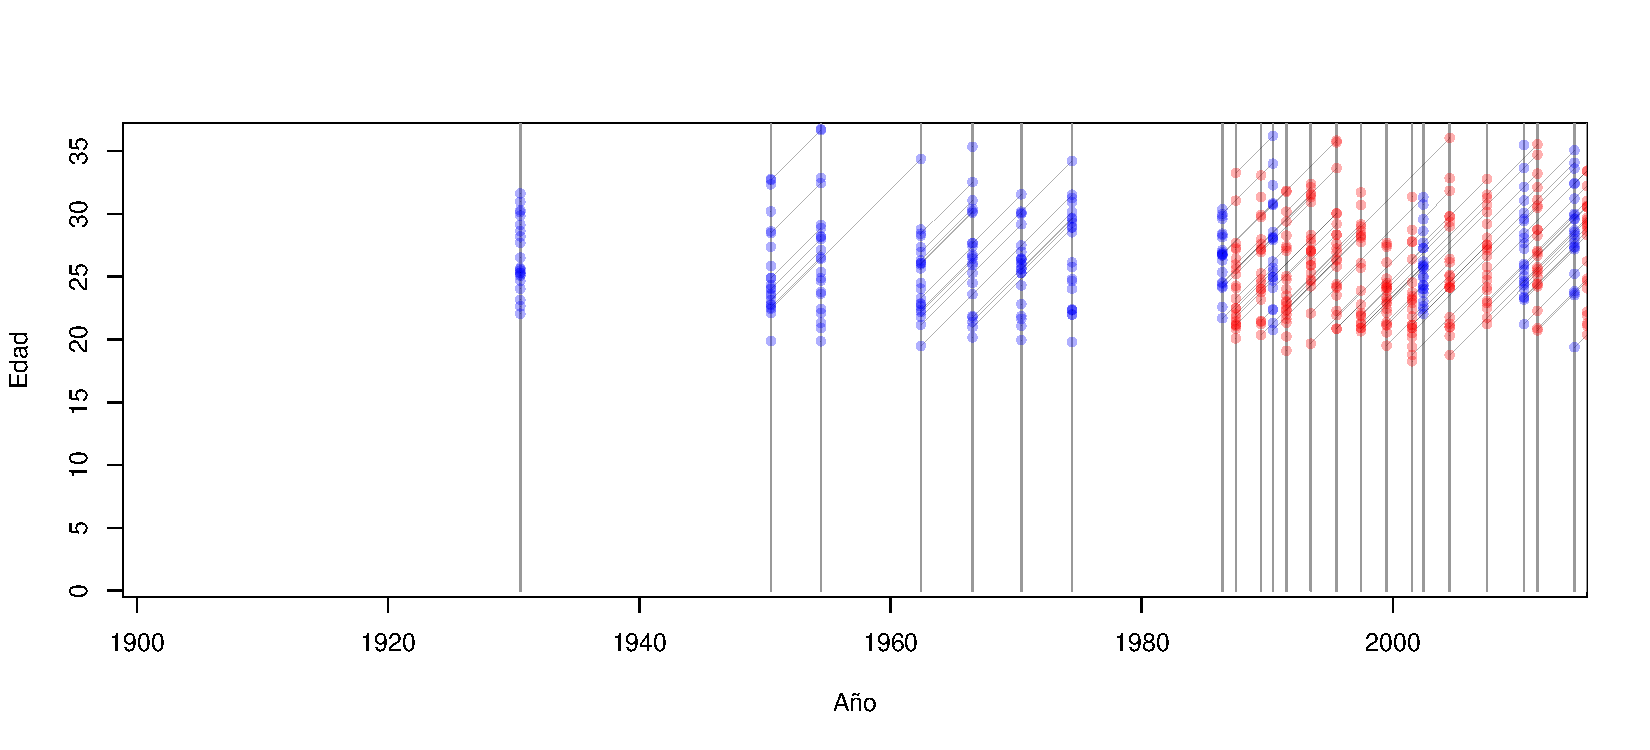
\includegraphics[scale=.88]{Figures/LexisPlayers2.pdf}\\
%pro tip: se puede hacer lo mismo con encuestas panel
%\end{frame}
%
%-----------------------------------
\section{analogos}
\begin{frame}
\frametitle{otras relaciones como el EPC (APC)}
\hspace{2cm}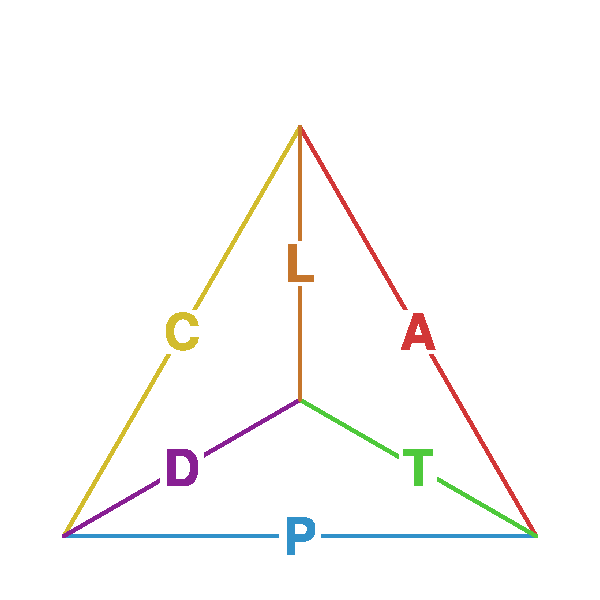
\includegraphics[scale=1.4]{Figures/TetraHedronEdgesOnly.pdf}\\
Riffe, Schoeley, \& Villavicencio (2015)
\end{frame}

\begin{frame}
\frametitle{el diagrama TAL}
\hspace{2cm}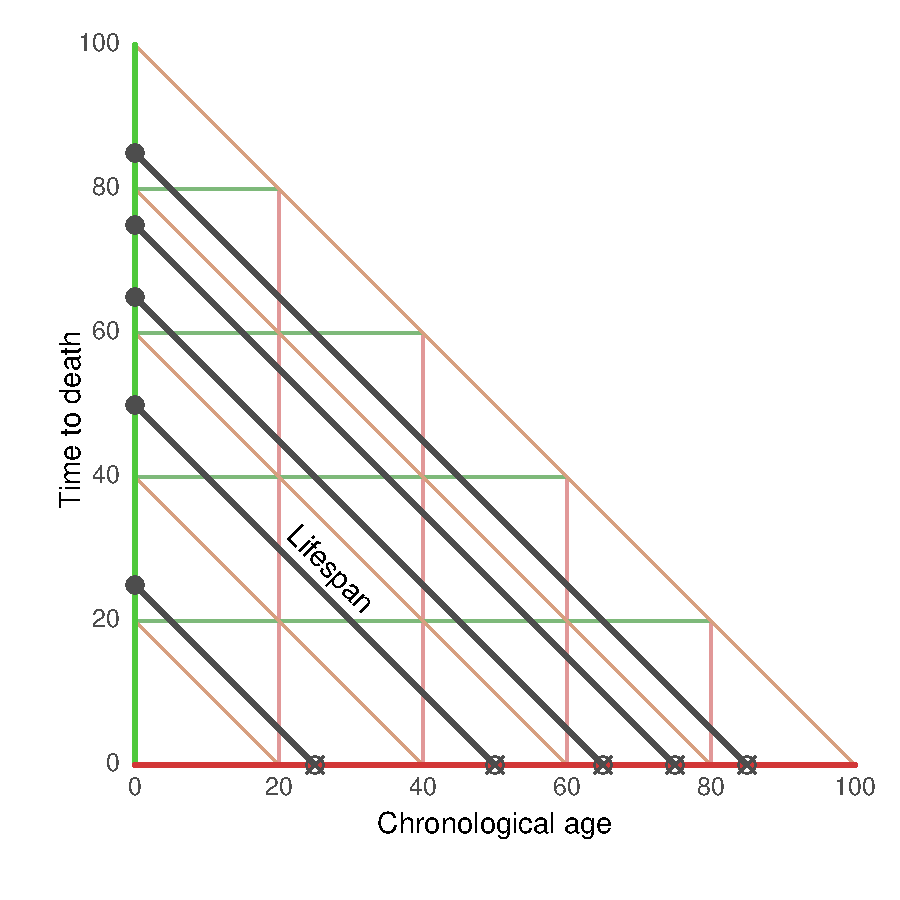
\includegraphics[scale=.9]{Figures/TALrt.pdf}\\
Riffe, Schoeley, \& Villavicencio (2015) \\ saltamos LCD y TPD \ldots
\end{frame}

\begin{frame}
\frametitle{aplicaci\'{o}n del diagrama TAL I}
\hspace{2cm}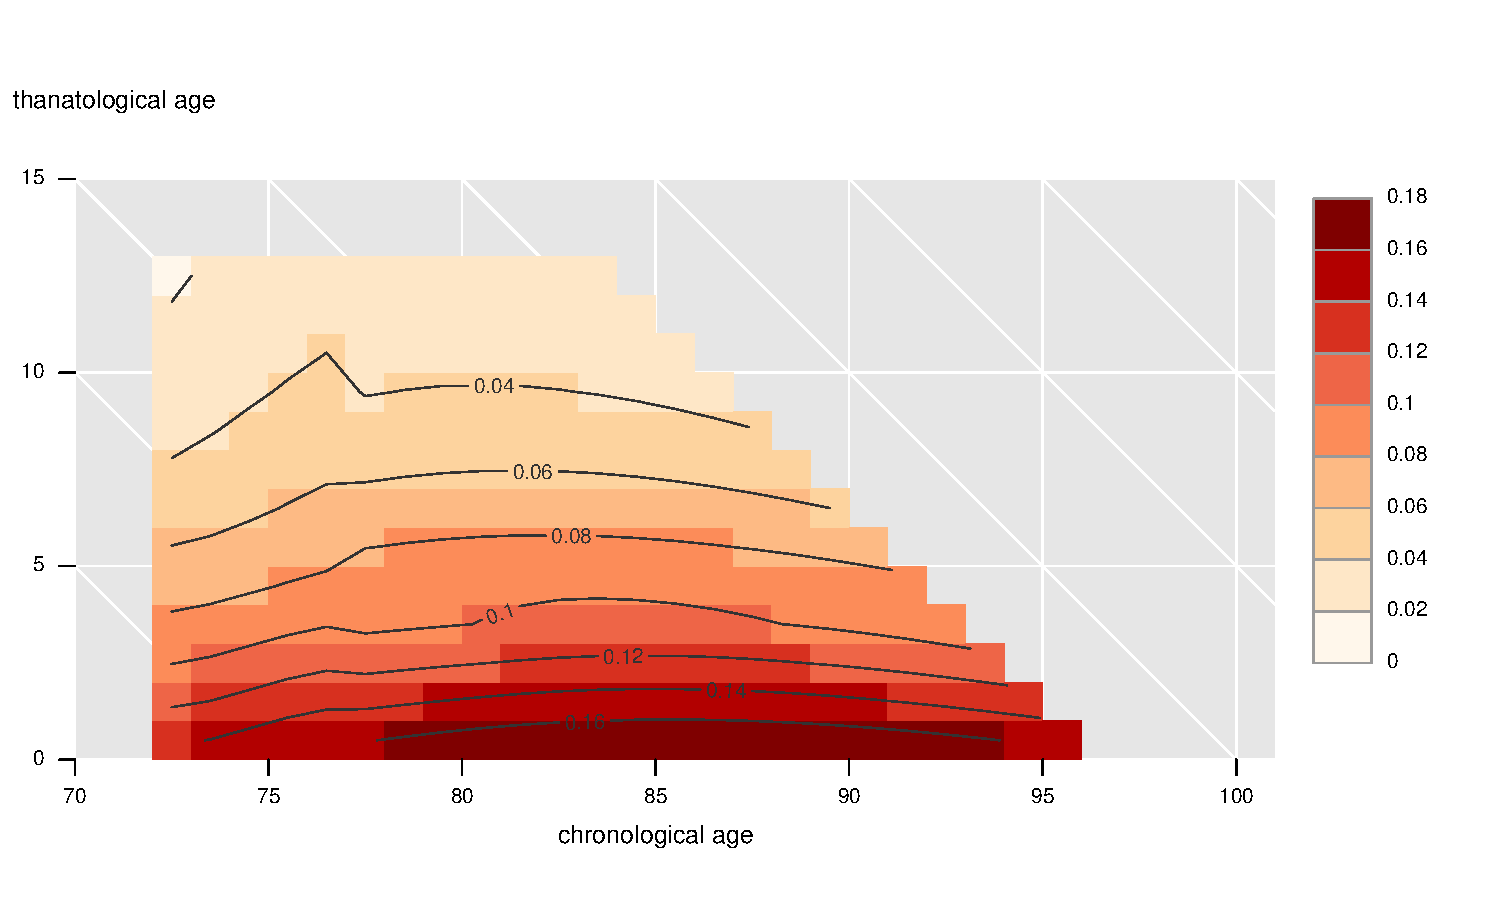
\includegraphics[scale=.9]{Figures/TAL_male_psych.pdf}\\
Riffe, Chung, Spijker, \& MacInnes (2016)
\end{frame}

\begin{frame}
\frametitle{aplicaci\'{o}n del diagrama TAL II}
\hspace{2cm}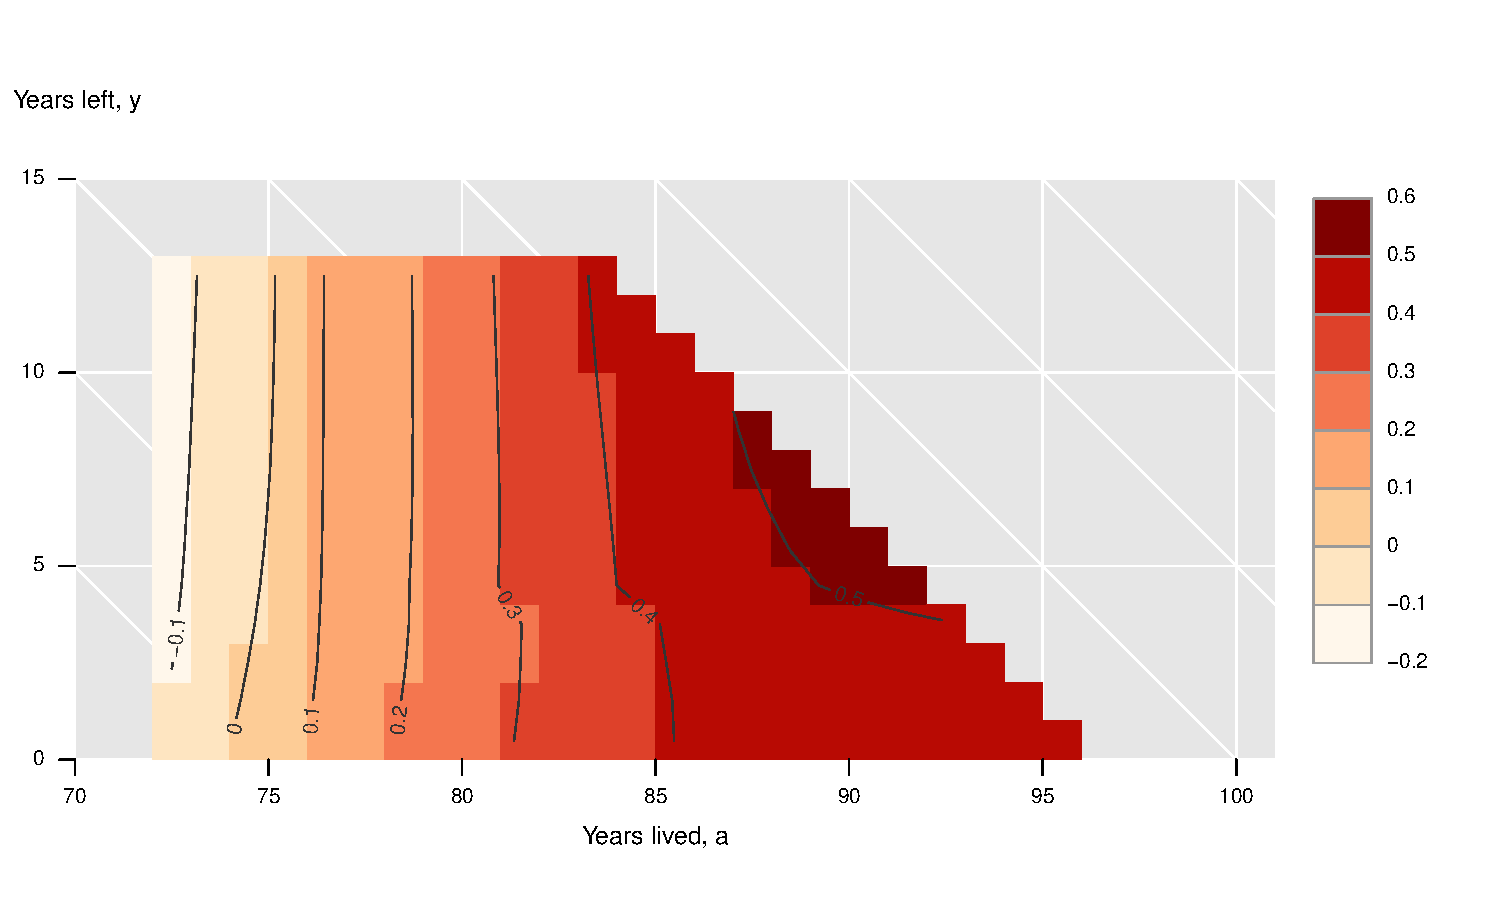
\includegraphics[scale=.9]{Figures/TAL_male_back.pdf}\\
Riffe, Chung, Spijker, \& MacInnes (2016)
\end{frame}

%-----------------------------------
\section{Transformations of Lexis}

\begin{frame}
\frametitle{Coordinate reprojection I}
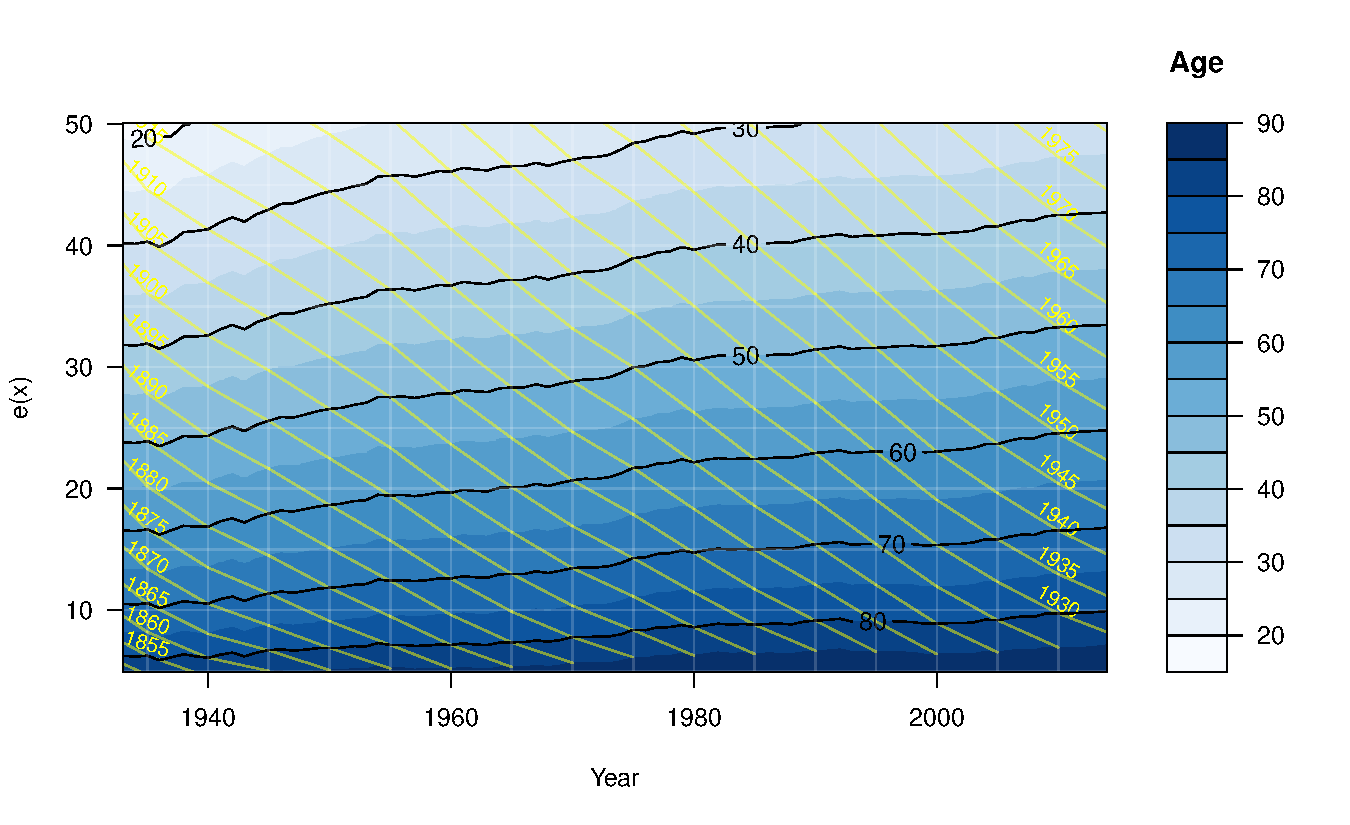
\includegraphics[scale=1]{Figures/ProspAgeLexis.pdf}\\
$age \rightarrow e(age)$, Riffe (2016)
\end{frame}

\begin{frame}
\frametitle{transformaciones de Lexis II}
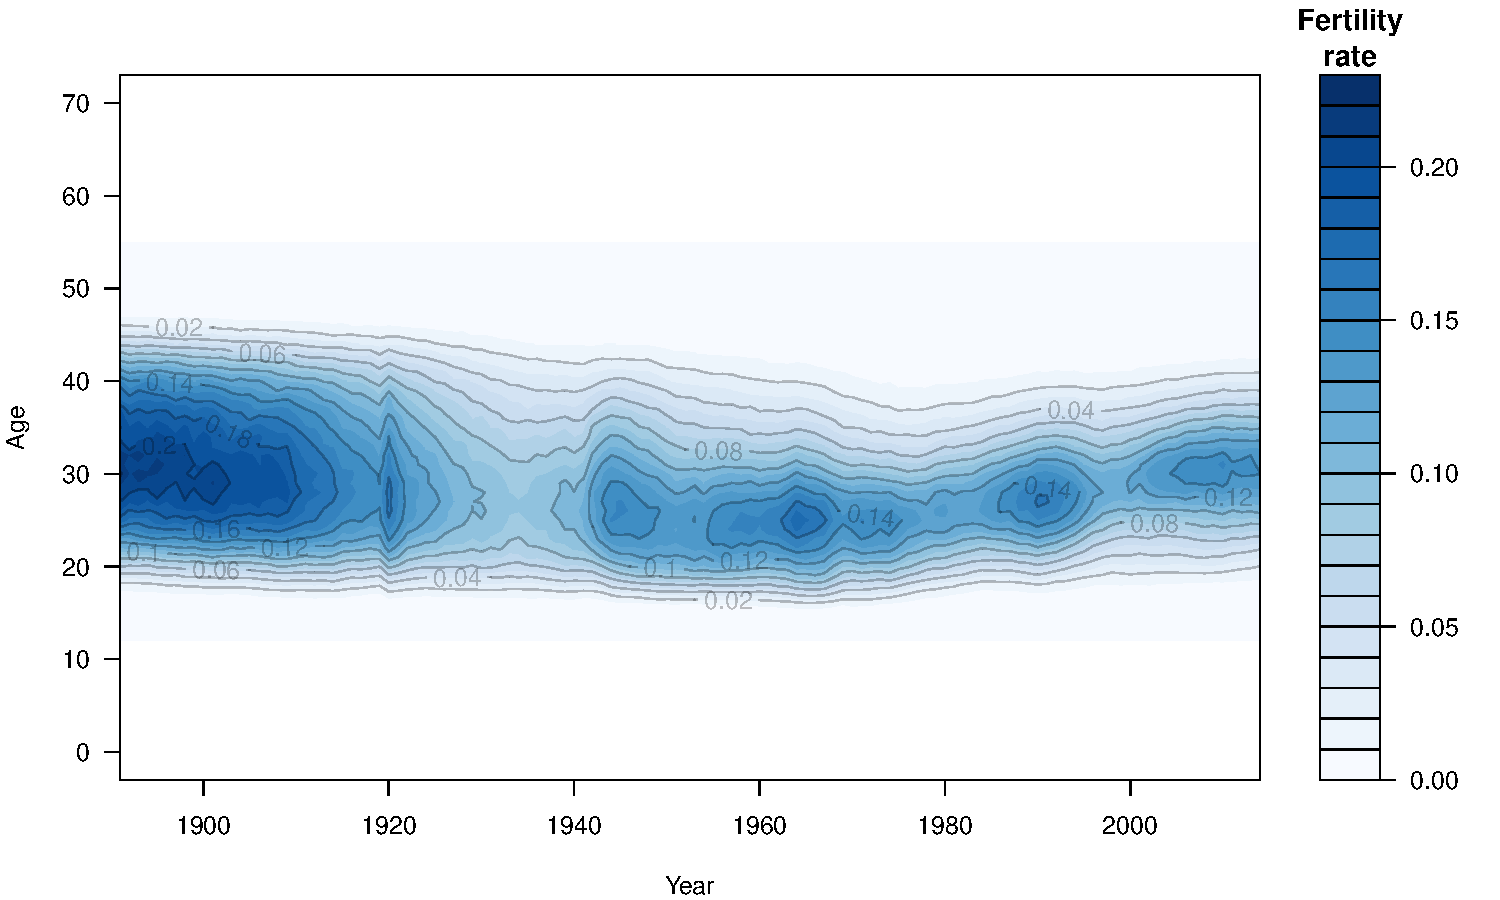
\includegraphics[scale=.9]{Figures/FertAPC.pdf}\\
Riffe (2016)
\end{frame}

\begin{frame}
\frametitle{transformaciones de Lexis III}
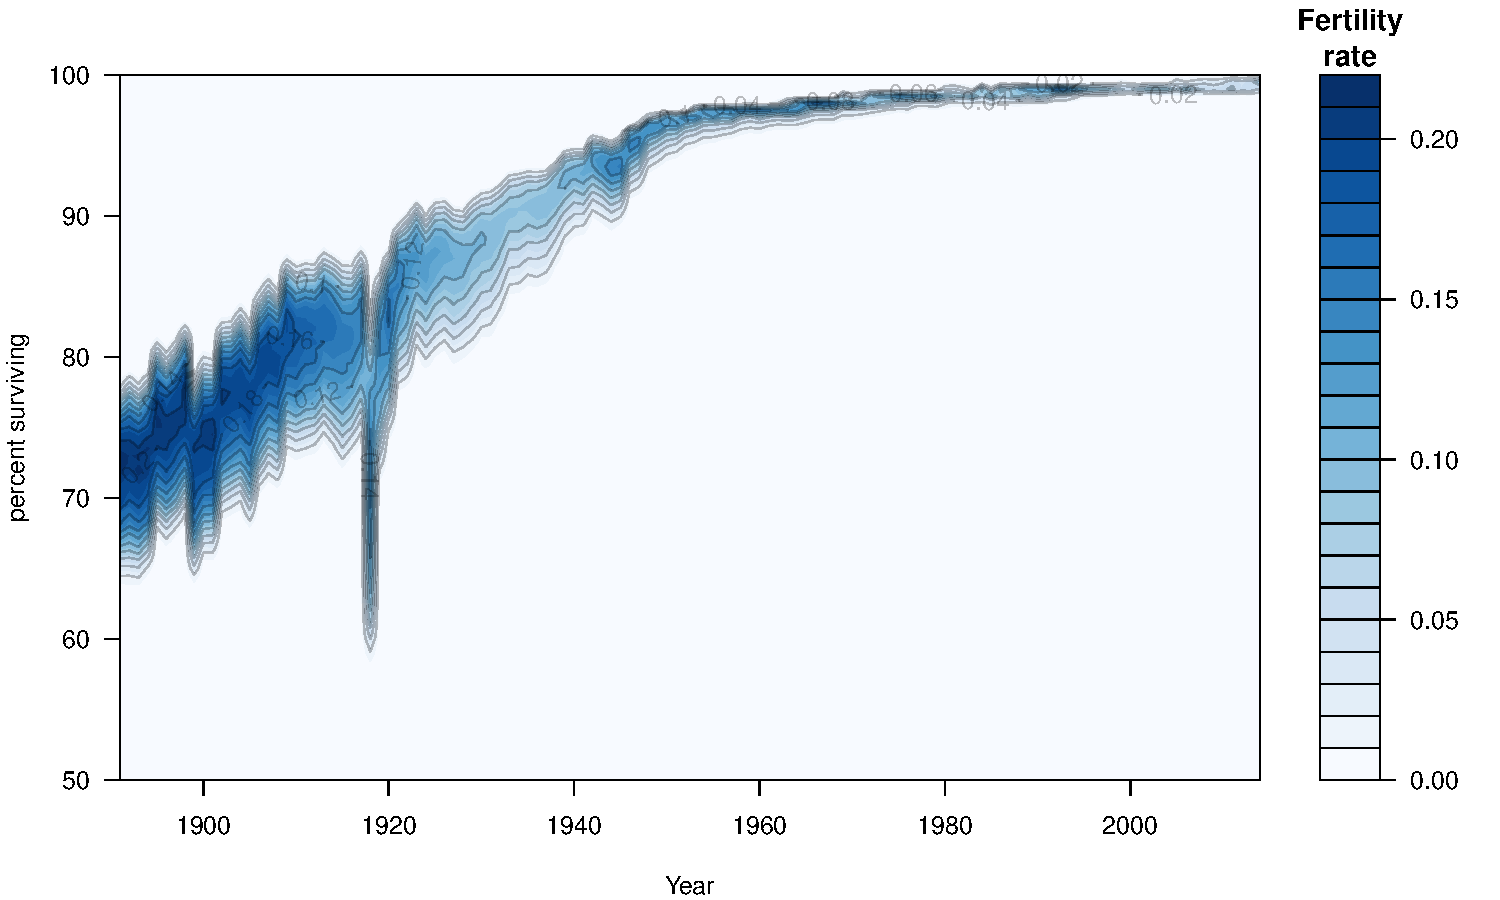
\includegraphics[scale=.9]{Figures/FertQuant.pdf}\\
Riffe (2016)
\end{frame}

%-----------------------------------
\section{resumen}
\begin{frame}
\frametitle{resumen}
\begin{itemize}[<+->]
  \item dese\~{n}o y explicaci\'{o}n de m\'{e}todos demogr\'{a}ficos
  \item visualizaci\'{o}n para:
  \begin{itemize}
    \item resumir la estructura de datos
    \item buscar anomolias que indican datos defectuosos
    \item detectar pautas de variaci\'{o}n en los datos
  \end{itemize}
  \item cambiar nacer o morir con entrar y salir
  \item aplicable con otros aspectos del tiempo demogr\'{a}fico (tiempo restante,
  duraci\'{o}n total)
  \item re-proyectar la superficie Lexis seg\'{u}n una transformaci\'{o}n demogr\'{a}fica
\end{itemize}
\end{frame}

% ---------------------------
\begin{frame}
\vspace{-15em}
\begin{center}
\hspace*{-6cm}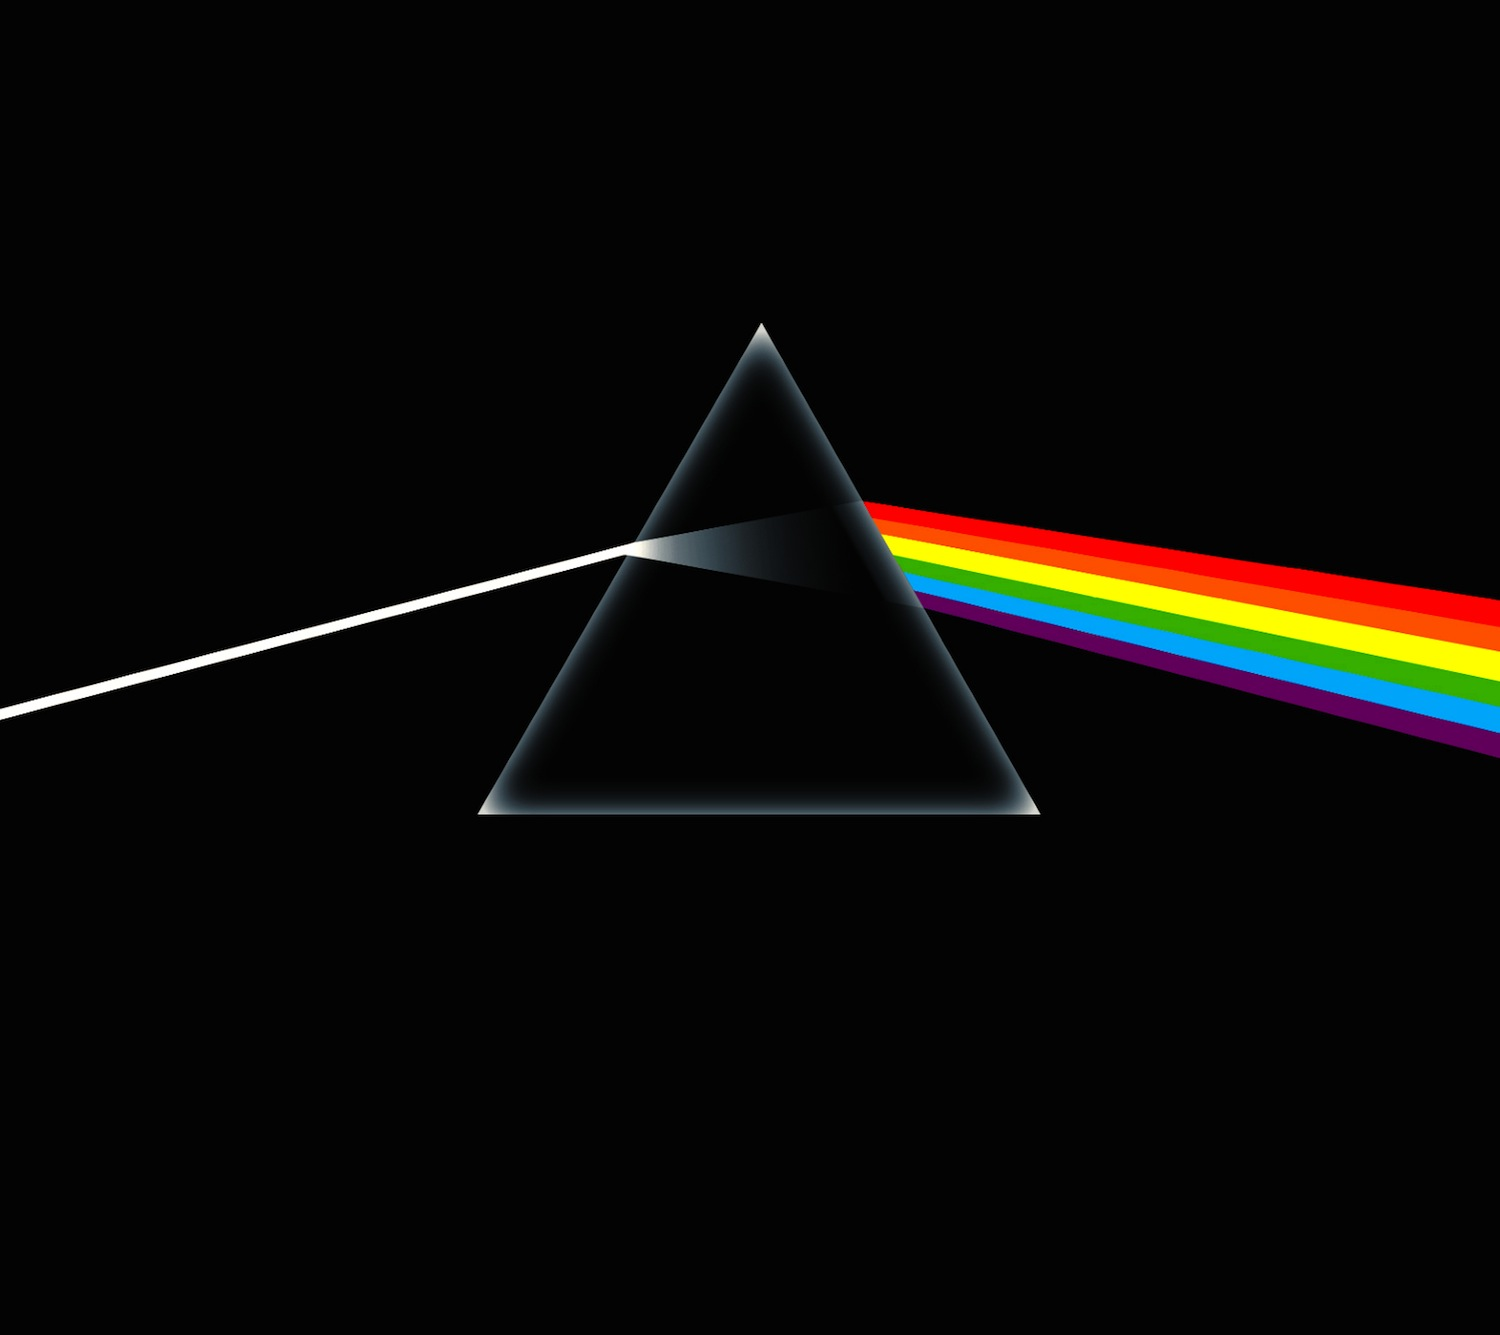
\includegraphics[scale=.7]{Figures/prism.jpg}
\end{center}
\end{frame}

\end{document}
